\chapter{Summary and Conclusions}
\label{cp.conc}

Over the previous century, astronomers have moved from manual observations to automated observatories, from solitary labs to worldwide collaborations, and from catalogs containing tens of thousands of stars to those containing millions. 
It is, therefore, not surprising that scholars have begun to experiment with data-driven and computationally intensive analysis methods. This dissertation demonstrates using one of these methods, namely Bayesian inference. 
This dissertation presents the application of Bayesian inference to estimate the significance of gravitational-wave candidates with intermediate-mass black holes. 
Even though no IMBHs were discovered, the approach supports the existence of eight stellar-mass binary black holes not previously reported in the first gravitational-wave transient catalog, GWTC-1. 
In addition, the thesis proposes a novel use of Bayesian model selection for diagnosing parameter estimation outcomes. 
The diagnostic method reveals that the first GW151226 analysis was incomplete: the method finds support for an asymmetric-mass merger, previously ignored. 
The thesis also proposes a phenomenological model for AGNs that may be used to estimate AGN parameters via hierarchical Bayesian inference. 
Simulation results reveal that more than 200 events with measurable spins are necessary to use this AGN population model -- potentially achievable by the end of the next LVK observing run. 
The preceding chapter describes the first catalog of TESS candidate exoplanet parameter estimates generated via Bayesian inference. 
In the future, this catalog may assist in confirming some TESS candidates as planets. 
Finally, the dissertation describes the software to accelerate inference, which can be costly. 
This software is utilized in this thesis and by the LVK collaboration for analyzing gravitational wave events using costly models.

In the final section of this dissertation, we briefly discuss future prospects in the gravitational wave and exoplanet domains. 

\paragraph{The future of GW -- LIGO and beyond}

\begin{figure}
\begin{center}
\centerline{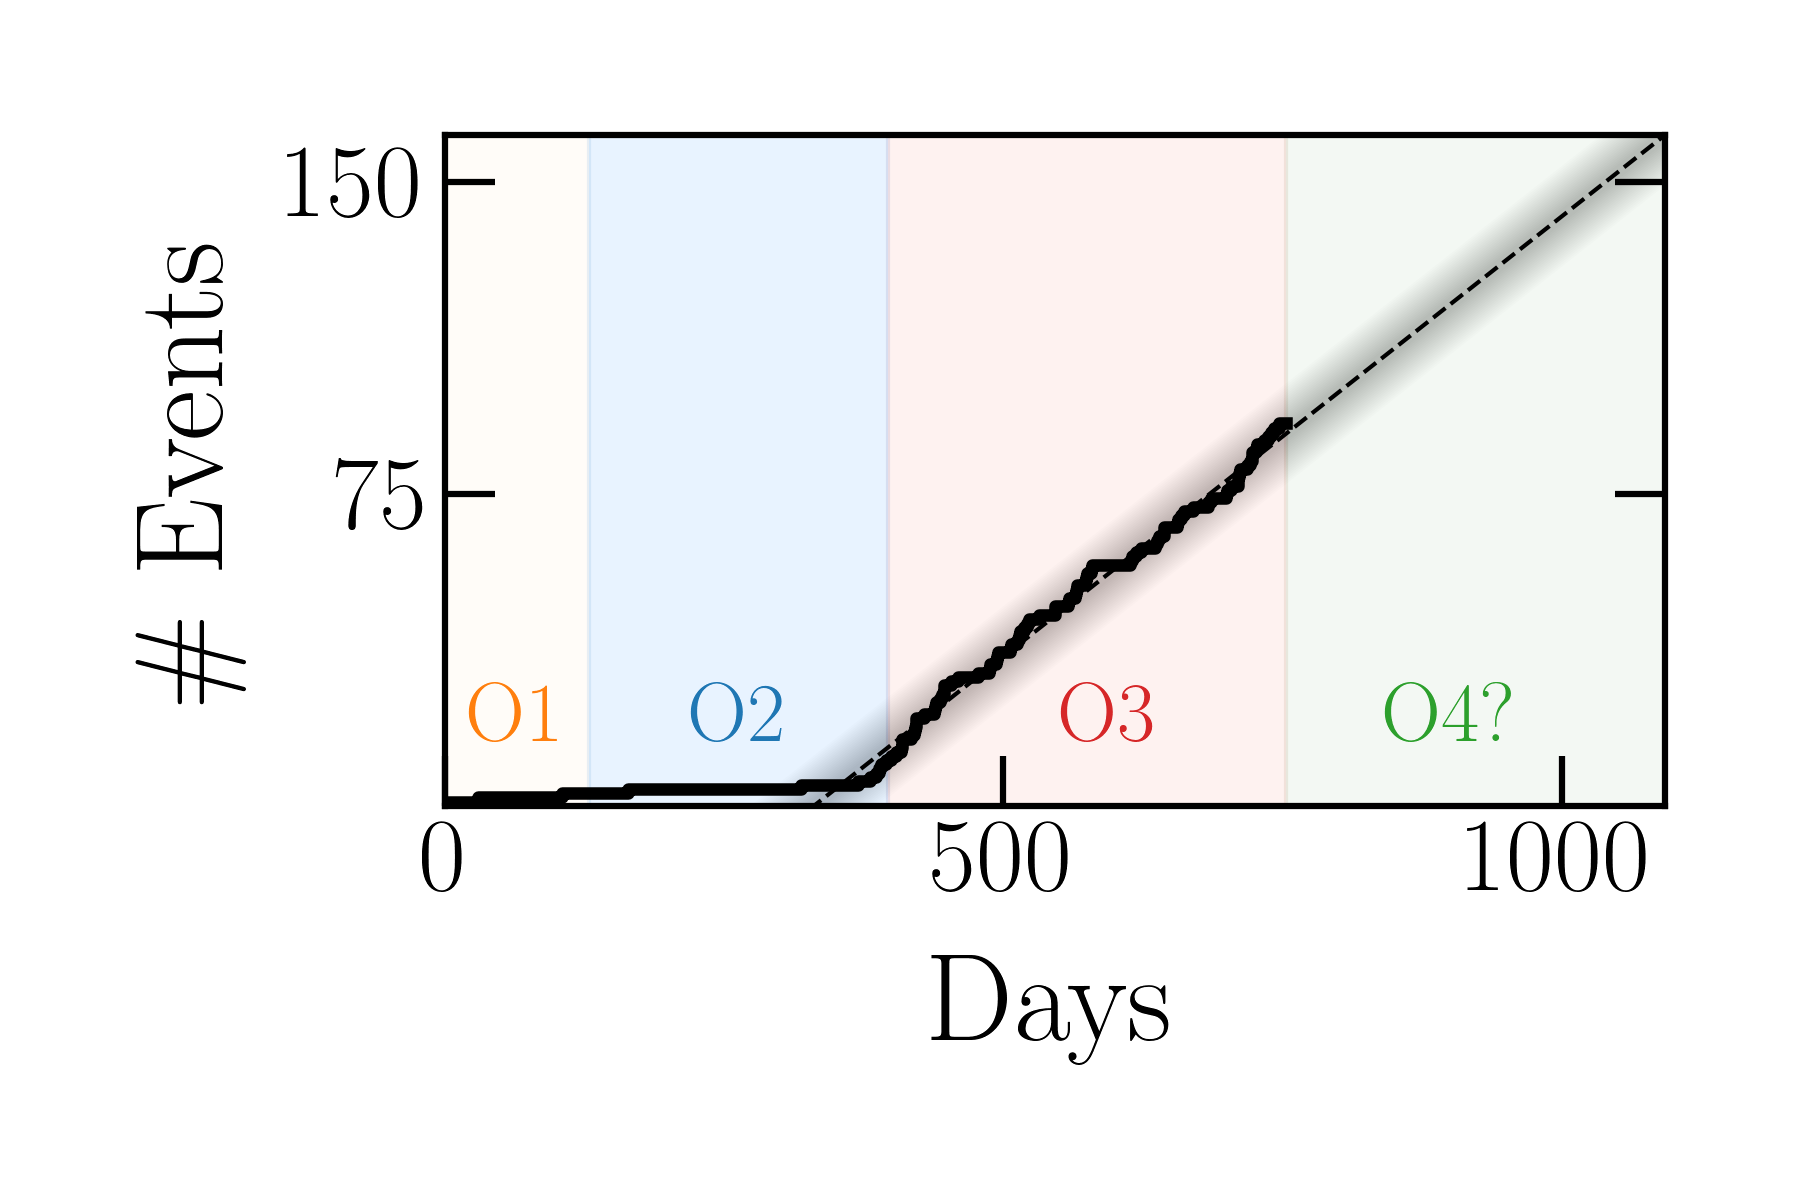
\includegraphics[width=1.\linewidth]{src/figures/gw_detection_timeframe.png}}
  \caption{\textbf{Cumulative Count of LVK Events:} The cumulative count of GW events on the vertical axis versus the number of observing days on the horizontal axis. O3 increased the count from 10 events to 93. The solid black curve is the true LVK cumulative count. The dashed black line represents an estimation of the increase in events during the fourth observing run (assuming that the O4 detection rate will be the same as O3's.  \github{https://github.com/avivajpeyi/cbc_gw_catalog_plotter}}
  \label{fig:accumulation_of_gw_events}
\end{center}
\end{figure}

The LIGO, VIRGO and KAGRA detectors have made GW astronomy a reality. 
Over the past eight years, the detections made have been a scientific goldmine. 
The detections have allowed us to study black hole mass spectrum~\cite{}, test general relativity~\cite{}, measure cosmological parameters~\cite{} and probe various neutron-star equation of state~\cite{}. 
Soon, the next LVK observing run, O4, will provide astronomers with more events two study the universe with. 
Figure~\ref{fig:accumulation_of_gw_events} shows the increase in GW events over the first three observing runs. 
It also provides a conservative estimate of the number of events in O4 (more detections are expected due to the detector upgrades).
However, even with the events that might be detected by the end of O4 and O5, the current GW detectors can only provide a glimpse of the full gravitational-wave universe. 

The next generation  of detectors will broaden this view. 
Plans of ground based detectors such as CE (Cosmic Explorer) and ET (Einstein Telescope), and even the spaced based detector LISA(Laser Interferometer Space Antenna) have been progressing in a positive direction. 
LISA will permit gravitational wave astronomers to study an entirely new spectrum of gravitational waves. 
For example, LISA will allow us to probe the merger of massive and supermassive black holes, and inspirals of compact objects such as white dwarf stars and neutron stars. 
The next generation ground based detectors (XG) will probe the same gravitational wave spectrum as the current LVK detectors. 
However, the XG detectrs will be over ten times more sensitive than the current detectors~\cite{}. 
Figure~\ref{fig:ligo_vs_ce} compares the sensitivity of CE and LIGO A+ (advanced LIGO). 
As shown in Figure~\ref{fig:ligo_vs_ce}a while the maximum distance the LIGO A+ can probe is $z\sim10$, CE can probe gravitational-wave astronomy from the edge of the observable universe $z\sim100$. 
This will allow astronomers to study the black hole mass spectrum as a function of redshift, and possible find primordial black holes.
\begin{figure}
\begin{center}
  \centerline{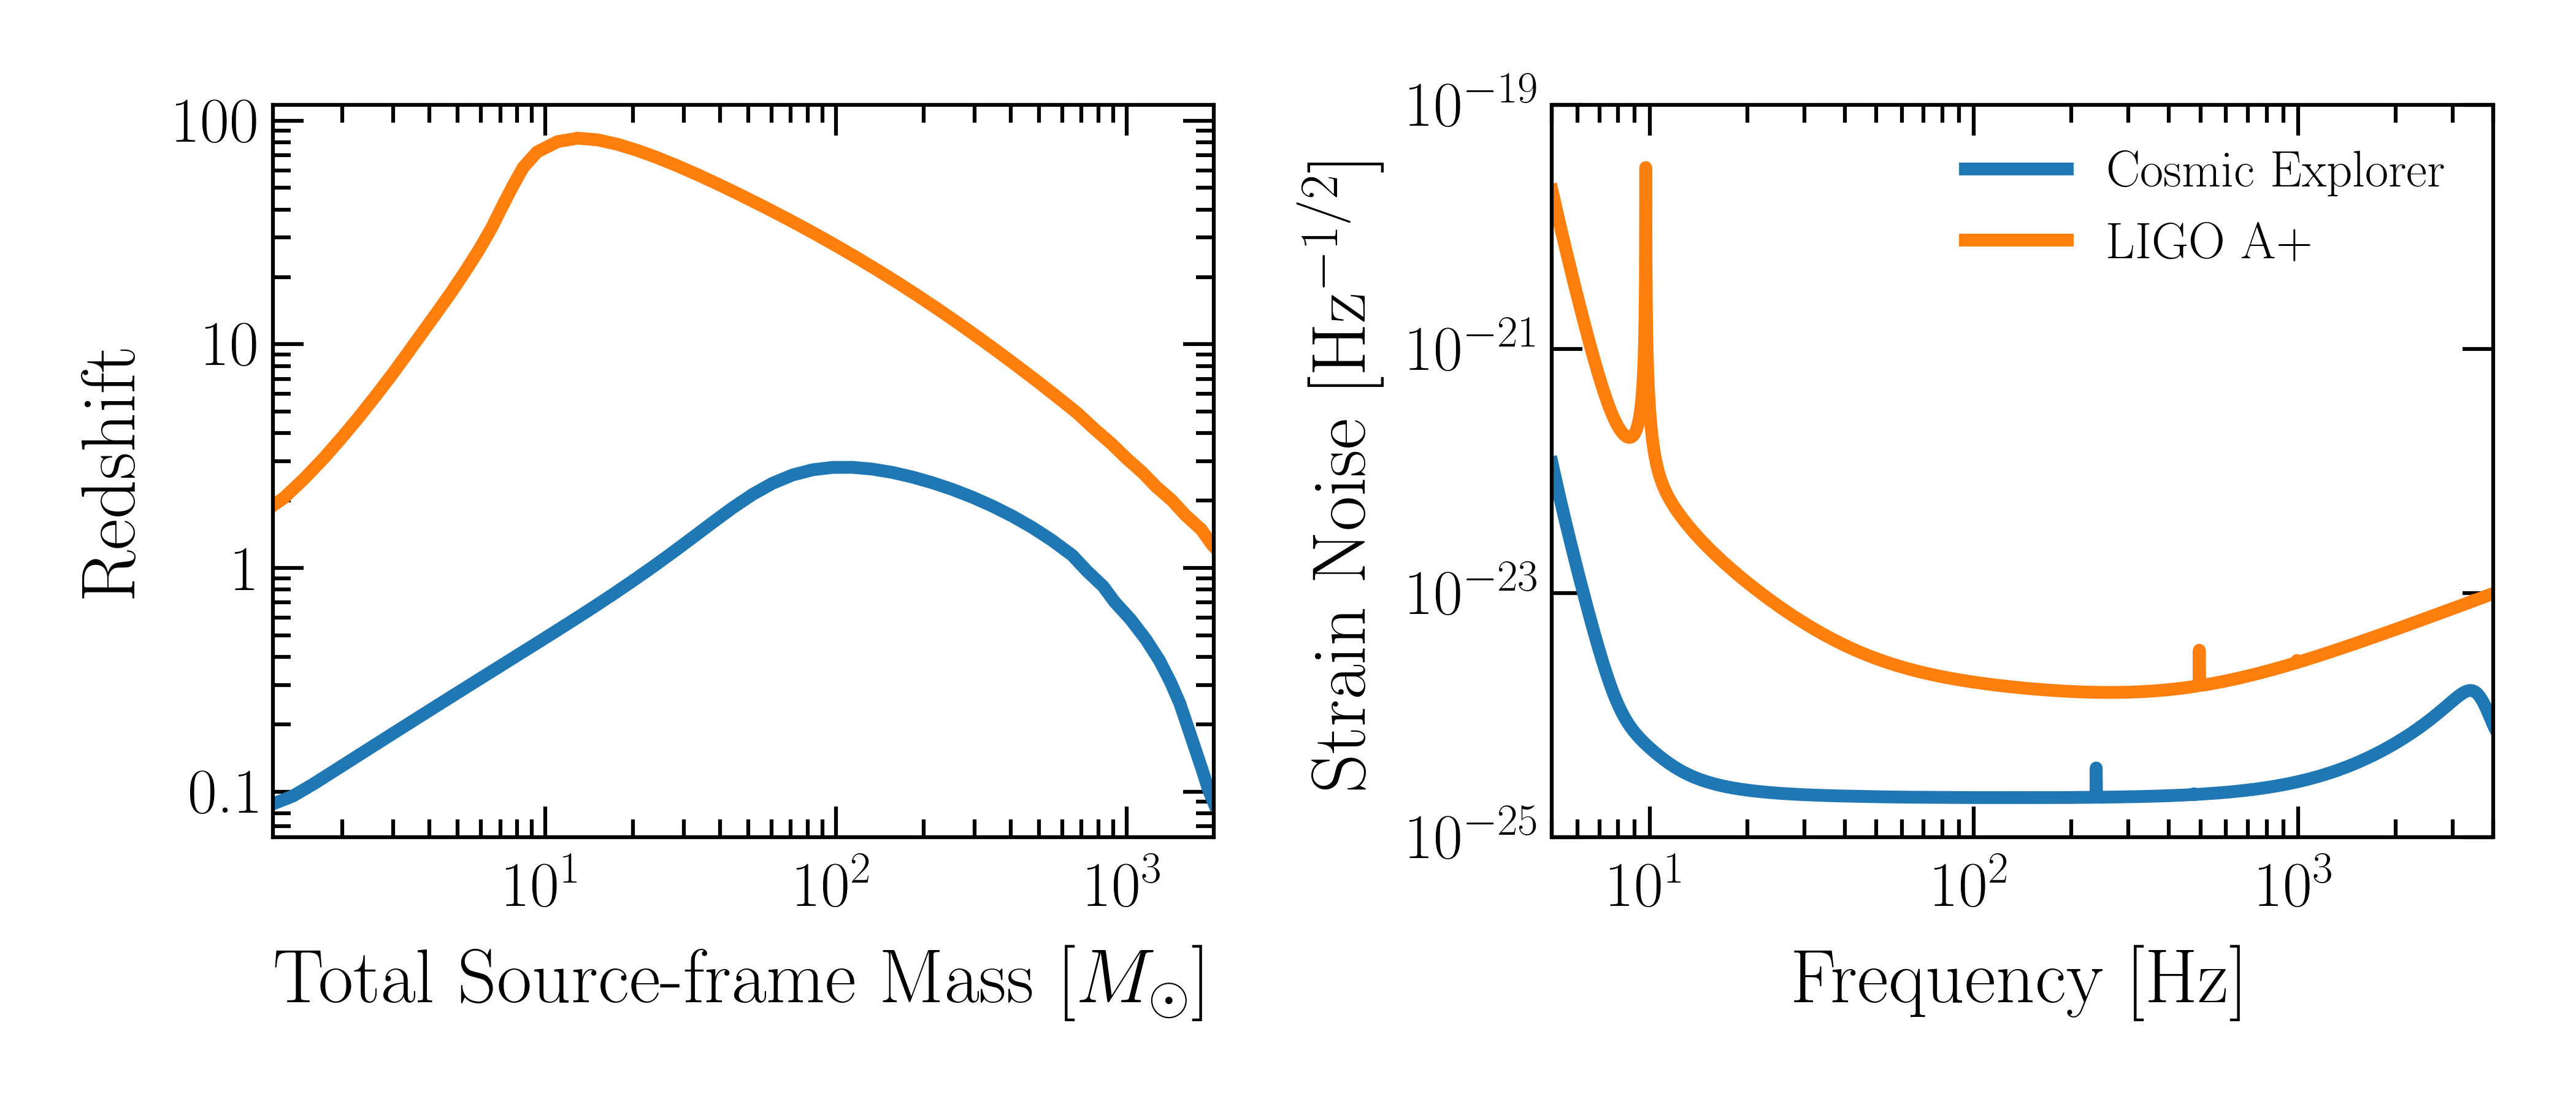
\includegraphics[width=1.\linewidth]{src/figures/ligo_vs_ce.png}}
  \caption{\textbf{LIGO A+ and CE Comparisons:}  \github{https://github.com/avivajpeyi/cbc_gw_catalog_plotter}}
  \label{fig:ligo_vs_ce}
\end{center}
\end{figure}


\paragraph{Probing habitable exoplanet atmospheres}
The next frontier for inquiry is characterizing the atmospheres of exoplanets. 
It's the next step toward finding life. 
Exoplanets have a similar driver larger than pure scientific curiosity. 
The ultimate goal
for many researchers is the search for habitable exoplanets. 
The exoplanet atmosphere
is the only way to infer whether or not a planet is habitable or likely inhabited; the
planetary atmosphere is our window into temperatures, habitability indicators, and
biosignature gases.


% https://www.annualreviews.org/doi/full/10.1146/annurev-astro-112420-020055

The Nancy Grace Roman Space Telescope, expected to launch in 2027, will make new exoplanet discoveries using a variety of methods. The ESA (European Space Agency) mission ARIEL, launching in 2029, will observe exoplanet atmospheres; a piece of NASA technology aboard, called CASE, will help zero in on exoplanet clouds and hazes

% The James Webb Space Telescope, which was not built to study exoplanets but to look for the oldest stars in the universe, has already delivered a string of breakthroughs in exoplanet research, including detecting carbon dioxide and water in the atmospheres of several of them. Quanz, however, cautions that Webb, although the most powerful observatory ever put to space, is not quite powerful enough to be able to see the much smaller, Earth-like planets that orbit closer to their stars at distances where liquid water can exist.



% Now that we have found exoplanets, the next frontier for inquiry is characterizing the atmospheres of exoplanets.
% +
% +Characterizing the atmospheres of exoplanets is the next frontier for inquiry because it allows us to learn more about the conditions on those planets. By studying the atmospheric composition, we can learn about the planet's climate and potential habitability. Additionally, studying the atmospheres of exoplanets can help us to better understand how planets form and evolve.

% The goal is to use TESS data to hopefully identify a possible "Goldilocks" situation: an exoplanet similar to Earth, in an orbit at which position liquid water could exist on the surface, and thus which could have the basics for life to develop. We're still a long way from being able to visit such exoplanets, but TESS' data has already helped develop a shortlist of potential candidates.

% Read More: https://www.slashgear.com/after-two-astonishing-years-nasas-tess-is-onto-the-next-exoplanet-hunt-11633044/?utm_campaign=clip


Wolszczan, who still searches for exoplanets as a professor at Penn State, says we’re opening an era of discovery that will go beyond simply adding new planets to the list. The Transiting Exoplanet Survey Satellite (TESS), launched in 2018, continues to make new exoplanet discoveries. But soon powerful next-generation telescopes and their highly sensitive instruments, starting with the recently launched James Webb Space Telescope, will capture light from the atmospheres of exoplanets, reading which gases are present to potentially identify tell-tale signs of habitable conditions.

The Nancy Grace Roman Space Telescope, expected to launch in 2027, will make new exoplanet discoveries using a variety of methods. The ESA (European Space Agency) mission ARIEL, launching in 2029, will observe exoplanet atmospheres; a piece of NASA technology aboard, called CASE, will help zero in on exoplanet clouds and hazes.


% https://www.nasa.gov/feature/jpl/cosmic-milestone-nasa-confirms-5000-exoplanets